\documentclass[tikz,border=12pt]{standalone}
\usepackage[T1]{fontenc}
\usepackage{xcolor}
\usetikzlibrary{positioning}

\begin{document}
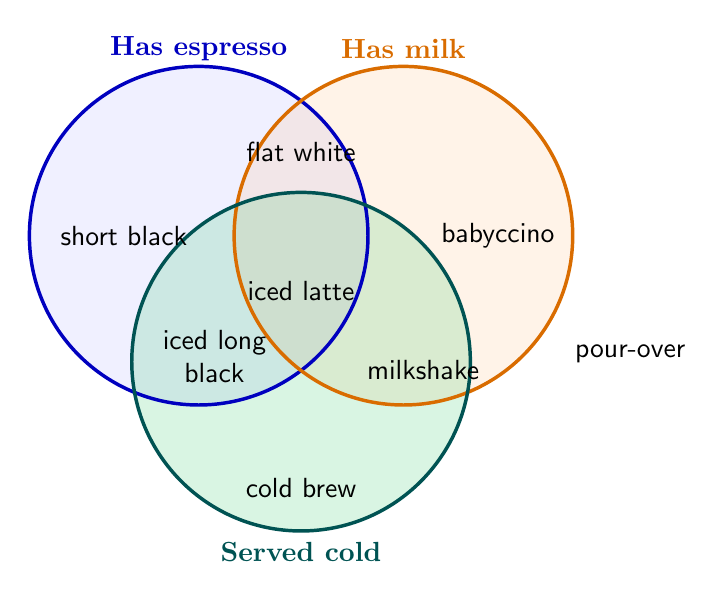
\begin{tikzpicture}[font=\sffamily]
  % Three gently overlapping sets
  \fill[blue!45, fill opacity=0.13] (-1.3,0.65) circle (2.15);
  \fill[orange!70, fill opacity=0.13] (1.3,0.65) circle (2.15);
  \fill[teal!55!green, fill opacity=0.15] (0,-0.95) circle (2.15);
  \draw[blue!75!black, line width=1.25pt] (-1.3,0.65) circle (2.15);
  \draw[orange!85!black, line width=1.25pt] (1.3,0.65) circle (2.15);
  \draw[teal!65!black, line width=1.25pt] (0,-0.95) circle (2.15);

  % Set labels
  \node[blue!75!black,font=\bfseries] at (-1.3,3.02) {Has espresso};
  \node[orange!85!black,font=\bfseries] at (1.3,3.02) {Has milk};
  \node[teal!65!black,font=\bfseries] at (0,-3.36) {Served cold};

  % Region labels
  \node[align=center] at (-2.25,0.65) {short black};
  \node[align=center] at (0,1.72) {flat white};
  \node[align=center] at (2.5,0.65) {babyccino};
  \node[align=center] at (-1.1,-0.88) {iced long\\black};
  \node[align=center] at (0,-0.05) {iced latte};
  \node[align=center] at (1.55,-1.05) {milkshake};

  % Outside all three sets
  \node[align=center] at (0,-2.55) {cold brew};
  \node[align=center] at (4.18,-0.85) {pour-over};
\end{tikzpicture}
\end{document}
